\RequirePackage[orthodox]{nag}
\documentclass[11pt]{article}

%% Define the include path
\makeatletter
\providecommand*{\input@path}{}
\g@addto@macro\input@path{{include/}{../../include/}}
\makeatother

\usepackage{../../include/akazachk}

\title{Simulation for Sustainable Systems}
\author{Andres Espinosa}
\begin{document}
\pgfplotsset{compat=1.18}
\maketitle

\tableofcontents
\section{Mock Exam}
\subsection{Part A}
This Petri Net has 4 places and 4 transitions, with only one token at the beginning.

\textbf{Post Matrix: }
\begin{align}
    I^{+} =
  \begin{bmatrix}
     0 & 0 & 1 & 1 \\
     1 & 0 & 0 & 0 \\
     0 & 1 & 0 & 0 \\
     0 & 0 & 1 & 0 
  \end{bmatrix}
\end{align}

\textbf{Pre Matrix: }
\begin{align}
    I^{-}
  \begin{bmatrix}
     1 & 1 & 0 & 0 \\
     0 & 0 & 1 & 0 \\
     0 & 0 & 0 & 1 \\
     0 & 0 & 0 & 0 
  \end{bmatrix}
\end{align}

\textbf{Incidence Matrix: }
\begin{align}
    C = 
  \begin{bmatrix}
     -1 & -1 & 1 & 1 \\
     1 & 0 & -1 & 0 \\
     0 & 1 & 0 & -1 \\
     0 & 0 & 1 & 0 
  \end{bmatrix}
\end{align}

\subsection{Part B}
Here I will define $M_0 = (1,0,0,0), M_1 = (0,1,0,0), M_2 = (0,0,1,0), M_3 = (0,0,0,1)$ and use them as shorthand for returns
\begin{center}
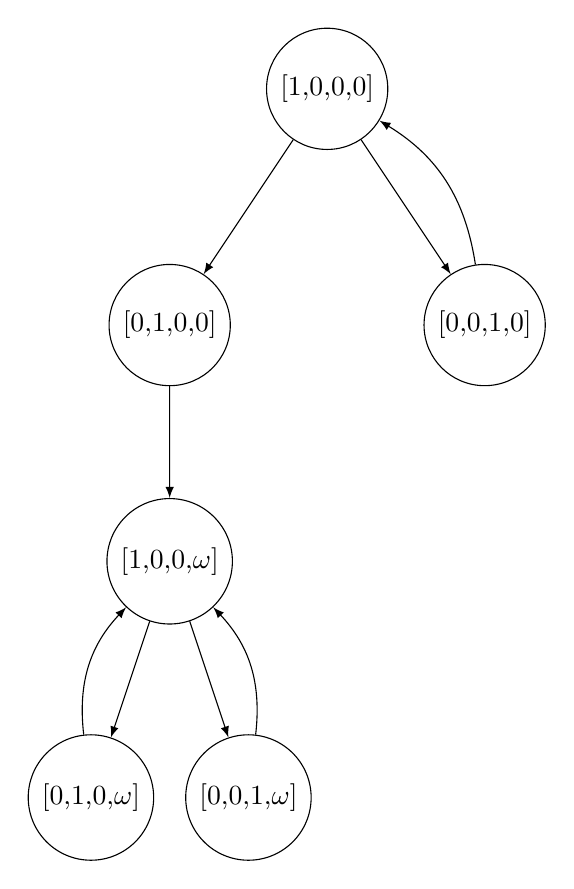
\begin{tikzpicture}[
    level distance=3cm,
    level 1/.style={sibling distance=4cm},
    level 2/.style={sibling distance=2cm},
    every node/.style={circle, draw, minimum size=0.8cm},
    edge from parent/.style={draw, -latex}
]

\node (root) {[1,0,0,0]}
    child {node (n1) {[0,1,0,0]}
        child {node (n3) {[1,0,0,$\omega$]}
            child {node (n4) {[0,1,0,$\omega$]}}
            child {node (n5) {[0,0,1,$\omega$]}}
        } 
    }
    child {node (n2) {[0,0,1,0]}
    };

% BACK EDGE
\draw[-latex, bend right=25] (n2) to (root);
\draw[-latex, bend left=25] (n4) to (n3);
\draw[-latex, bend right=25] (n5) to (n3);

\end{tikzpicture}
\end{center}
% I should fix this to add the transitions to the edges and add edges back to the previous states they come from.



\subsection{Part C}
N is not bounded, as a result of $p_4$, which can consume tokens indefinitely.

\subsection{Part D}
Completed in Python and verified in Python, the resulting P and T invariant vectors are:
\begin{align}
  P = 
  \begin{bmatrix}
     1 \\ 1 \\ 1 \\ 0
  \end{bmatrix},
  \quad T =
  \begin{bmatrix}
    0 \\ 1 \\ 0 \\ 1
  \end{bmatrix}
\end{align}

\subsection{Part E}
\begin{equation}
    \textbf{p}^\top \textbf{m} = m_1 + m_2 + m_3 = 1
\end{equation}
It is a necessary and sufficient condition, as the possible markings reachable from $M_0$ is (0,1,0,0) and (0,0,1,0).

\subsection{Part F}
The net does not terminate since there can be infinite firing into $p_4$.

\subsection{Part G}
The net is indeed live.
From the coverability graph we can see that from any node there is a path to the original position.


\end{document}